\chapter{Brief introduction to deep learning}\label{sec:deep_learning}
Deep learning is a subfield of machine learning that focuses on the development and application of complex structures called artificial neural networks (ANN) composed by multiple layers of learning.
The idea behind ANNs origins from connectionism research trying to understand and reproduce the human brain using mathematical models; this is the reason why they have this name.
ANNs represent the leading method that brings artificial intelligence on the rise in the last years, surpassing other classical machine learning techniques and achieving extraordinary results in many fields, commonly associated to human intelligence only, like natural language processing \cite{bengio2000neural}, speech recognition \cite{hinton2012deep}, computer vision \cite{krizhevsky2012imagenet}, autonomous driving \cite{grigorescu2020survey}, medical diagnosis \cite{gulshan2016development} and many others.

The basic theory and principles behind ANNs were developed more than 50 years ago, starting from the perceptron model by \citeauthor{rosenblatt1958perceptron} \cite{rosenblatt1958perceptron}, but research on this field exploded in the last years due to the high computational resources and amount of data required to properly train a model that were simply not available before.

In the following sections we give an introduction of the main principles allowing an ANN to learn how to solve a task, focusing mostly on the techniques used in this work to improve the learning process, namely transfer learning and knowledge distillation.
However, a comprehensive description of deep learning is out of scope of this work; more information can be found in the very large amount of papers available in the literature and in authoritative reviews on the topic, such as in \cite{lecun2015deep}.


\section{From artificial neurons to learning}
\subsection{Neural architecture}
\begin{figure}
    \centering
    \begin{subfigure}[b]{0.6\textwidth}
        \resizebox{\textwidth}{!}{ \begin{tikzpicture}[
    scale=1.2,
    basic/.style={draw,fill=none,text badly centered,minimum width=3em},
    circ/.style={basic,circle,minimum width=3em},
    square/.style={basic,regular polygon,regular polygon sides=4,minimum width=2em},
    func/.style={basic,circle, minimum width=3.5em}
]
    %inputs
    \node[circ] (x1) {$x_1$};
    \node[circ,below of=x1,yshift=-1em] (x2) {$x_2$};
    \node[circ,below of=x2,yshift=-1em] (x3) {$x_3$};
    \node[below of=x3,yshift=0.2em] (dots) {\vdots};
    \node[circ,below of=dots,yshift=-0.2em] (xn) {$x_n$};

    \node[square,right of=x1,xshift=6em] (bias) {1};

    \node[func,right of=x3,xshift=6em] (sum) {\large$\sum$};
    \node[below of=sum,yshift=-0.6em] {$\sum\limits_{i=1}^n w_ix_i + b$};

    \node[square,right of=sum,xshift=4em] (activation) {
        \begin{tikzpicture}
            \draw (0em,1em) -- (0em,-1em) (-1em,0em) -- (1em,0em) % axis
                  (-0.1em,0.8em) -- (0em,1em) (0em,1em) -- (0.1em,0.8em) % y arrow
                  (0.8em,-0.1em) -- (1em,0em) (1em,0em) -- (0.8em,0.1em); % x arrow
            \draw[line width=1.5pt] (-1em,0) -- (0,0) (0,0) -- (0.75em,0.75em); % ReLU
        \end{tikzpicture}
    };

    \draw[->] (x1) -- (sum) node [pos=0.5,above,font=\footnotesize] {$w_1$};
    \draw[->] (x2) -- (sum) node [pos=0.5,above,font=\footnotesize] {$w_2$};
    \draw[->] (x3) -- (sum) node [pos=0.5,above,font=\footnotesize] {$w_3$};
    \draw[->] (xn) -- (sum) node [pos=0.5,above,font=\footnotesize] {$w_n$};
    \draw[->] (bias) -- (sum) node [pos=0.5,right,font=\footnotesize] {$b$};
    \draw[->] (sum) -- (activation);
    \draw[->] (activation) -- ++(1.5,0);
\end{tikzpicture} }
        \caption{Artificial neuron structure}
        \label{subfig:artificial_neuron}
    \end{subfigure}\hspace{2em}
    \begin{subfigure}[b]{0.3\textwidth}
        \resizebox{\textwidth}{!}{ 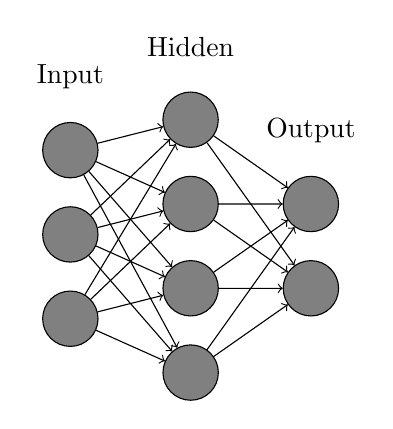
\begin{tikzpicture}[
    scale=1.2,
    basic/.style={draw,fill=gray,text badly centered,minimum width=2em},
    circ/.style={basic,circle,minimum width=2em},
]
    %inputs
    \node[circ] (i1) {};
    \node[circ,below of=i1,yshift=-0.2em] (i2) {};
    \node[circ,below of=i2,yshift=-0.2em] (i3) {};
    \node[above of=i1,yshift=-0.2em] {Input};

    \node[circ,right of=i1,xshift=1.5em,yshift=1.1em] (h1) {};
    \node[circ,below of=h1,yshift=-0.2em] (h2) {};
    \node[circ,below of=h2,yshift=-0.2em] (h3) {};
    \node[circ,below of=h3,yshift=-0.2em] (h4) {};
    \node[above of=h1,yshift=-0.2em] {Hidden};

    \node[circ,right of=h2,xshift=1.5em] (o1) {};
    \node[circ,right of=h3,xshift=1.5em] (o2) {};
    \node[above of=o1,yshift=-0.2em] {Output};

    \draw[->] (i1) -- (h1);
    \draw[->] (i1) -- (h2);
    \draw[->] (i1) -- (h3);
    \draw[->] (i1) -- (h4);
    \draw[->] (i2) -- (h1);
    \draw[->] (i2) -- (h2);
    \draw[->] (i2) -- (h3);
    \draw[->] (i2) -- (h4);
    \draw[->] (i3) -- (h1);
    \draw[->] (i3) -- (h2);
    \draw[->] (i3) -- (h3);
    \draw[->] (i3) -- (h4);

    \draw[->] (h1) -- (o1);
    \draw[->] (h1) -- (o2);
    \draw[->] (h2) -- (o1);
    \draw[->] (h2) -- (o2);
    \draw[->] (h3) -- (o1);
    \draw[->] (h3) -- (o2);
    \draw[->] (h4) -- (o1);
    \draw[->] (h4) -- (o2);
\end{tikzpicture} }
        \vspace{0.7em}
        \caption{A simple ANN}
        \label{subfig:simple_nn}
    \end{subfigure}
    
    \caption{(a) The basic structure of an artificial neuron and (b) a simple 3-layers feedforward ANN}
    \label{fig:artificial_neuron}
\end{figure}

The main unit composing an ANN is the artificial neuron.
The first artificial neuron was proposed by McCulloch and Pitts in 1943 \cite{McCulloch1943}.
Its generic structure is visible in figure \ref{subfig:artificial_neuron} and its output can be described by the following equation:
\begin{equation}
y = \varphi(\sum\limits_{i=1}^n w_ix_i + b)
\label{eqn:artificial_neuron}
\end{equation}
where $x_i$ are the input values, $w_i$ are the weights, $b$ is a bias term and $\varphi$ is the activation function.
In other words, the artificial neuron performs a linear combination of inputs $x$, weights $w$ and bias term $b$ and then applies a non-linearity using the function $\varphi$ to determine whether it should output a value based on the weighted sum of its inputs.
The correct values of weights that, given an input $x$, produce the desired output $y$ shall be found through learning.

The activation function shall be a differentiable function in order to apply common learning optimization methods, that are mentioned in \ref{sec:learning_process}.
The most used activation function is the rectified linear unit (ReLU) \cite{ramachandran2017searching} expressed by the equation:
\begin{equation}
    y = max(0, x)
    \label{eqn:relu}
\end{equation}

The network is usually formed by subsequent layers composed by multiple neurons, where the output of a layer is used as input of the following one; this structure is called feedforward ANN, since the flow of calculation is performed in a single forward direction forming an acyclic graph; other configurations are also possible that creates cycles like in recurrent neural networks \cite{lstm1997}.
An example of a 3-layers feedforward NN is depicted in figure \ref{subfig:simple_nn}. The first layer that receives external data is called \emph{input layer}, the last one that produces the results is called \emph{output layer}, all those between them are called \emph{hidden layers}.


\subsection{Learning Process} \label{sec:learning_process}
The goal of the learning process is to find the weights and bias values that allow to use the ANN to resolve a specific task whether it is a classification task, a regression or a different kind.
The task is represented as an optimization problem that consists of minimizing a loss function that measures the distance between the output calculated by the network $y_i$ and the expectation $\hat{y}_i$.
Most used loss functions are mean absolute error (MAE):
\begin{equation}
    MAE = \frac{1}{n} \sum\limits_{i=1}^n \mid y_i - \hat{y}_i \mid
    \label{eqn:mae}
\end{equation}
the mean squared error (MSE):
\begin{equation}
    MSE = \frac{1}{n} \sum\limits_{i=1}^n (y_i - \hat{y}_i)^2
    \label{eqn:mse}
\end{equation}
and for outputs that represent probability distributions cross entropy:
\begin{equation}
    H = - \sum\limits_{i=1}^n y_i \log \hat{y}_i
    \label{eqn:cross_entropy}
\end{equation}
and Kullback-Leibler divergence \cite{Kullback1951}:
\begin{equation}
    KLDiv = \sum_{i=1}^{N} \hat{y}_i log\frac{\hat{y}_i}{y{_i}}
    \label{eqn:kldiv}
\end{equation}

The process involves passing input training data through the network to calculate a prediction that is compared with the actual value, using the selected loss function; the gradient of the loss with respect to the weights and biases is then calculated using back-propagation \cite{rumelhart1986learning} layer by layer, starting from the output layer and moving backward to find how the weights and biases shall be changed to minimize the loss.
The network is then updated using an optimization strategy like stochastic gradient descent (SGD) or Adam \cite{kingma2014}, changing weights by little steps towards loss function decreasing direction, to find its minimum; the size of those steps is usually determined by a parameter called \emph{learning rate}.
The whole process is repeated for multiple iterations, or epochs, until the network prediction reliability is considered satisfactory enough or the network stops improving its performance.
It shall be considered that solutions to real-world problems are not trivial and the optimizer might not find the global minimum of the loss function, but instead get stuck in a local minima; to avoid this, learning rate and some other hyper-parameters can be tuned, but this requires many attempts and experience.


\section{Convolutional neural networks}
The usage of dense networks, i.e. ANNs composed by multiple fully-connected layers of neurons only, does not fit very well when the inputs are images: the high computational costs due to the size of the input layer and the lack of spatial correlation between pixels heavily limits the performance of ANN on images.
For this reason, convolutional neural networks (CNN) has been introduced.

Convolution is a mathematical operation that represents the amount of overlap of a function $g$ as it is shifted over another function $f$ \cite{wolfram_conv}.
Its discrete version where $f$ and $g$ are defined on integers set $\mathbb{Z}$ can be expressed as:
\begin{equation}
    (f * g)(n) = \sum\limits_{m=-\infty}^\infty f(m)g(n-m)
    \label{eqn:convolution}
\end{equation}

Convolution is widely used in image processing, it is performed adding to each pixel of an image the values of its neighbours weighted by the values of a matrix called kernel.
This operation transforms the original image and, based on the kernel used, can generate a blurred or a sharpen version of the image, can detect edges around objects or extract more complex features from the source.
In general, the kernel is used to represent or extract a specific feature of the image, e.g. lines, edges, circles, etc.
A kernel is a small, usually square, matrix specifically designed for a task, it is applied on the image starting from the first pixel on a corner and then shifted to cover the whole image; at each step the values of the pixel and its surrounding neighbours are multiplied by the corresponding values on the kernel and the results are then summed up to generate the output for the pixel.
An example of vertical edge detection kernel and its application is depicted in figure \ref{fig:convolution}.

\begin{figure}
    \centering
    \resizebox{0.8\textwidth}{!}{ \begin{tikzpicture}[
    mmat/.style={
        matrix of nodes,
        nodes in empty cells,
        column sep=-\pgflinewidth/2,
        row sep=-\pgflinewidth/2,
        cells={nodes={draw,inner sep=0.5em,thin,minimum width=2em,minimum height=2em}},
        draw=#1,
        thick,
        inner sep=0pt
    },
    mmat/.default=black,
    node distance=0.3em
]
  \matrix[mmat](src){
    0 & 0 & 0 & 0 & 2 & 0 & 0 & 0 \\
    0 & 0 & 0 & 0 & 2 & 0 & 0 & 0 \\
    0 & 0 & 0 & 1 & 2 & 2 & 0 & 0 \\
    0 & 0 & 1 & 1 & 2 & 2 & 0 & 0 \\
    0 & 0 & 1 & 1 & 2 & 0 & 0 & 0 \\
    0 & 0 & 1 & 2 & 2 & 0 & 0 & 0 \\
    0 & 0 & 1 & 2 & 2 & 0 & 0 & 0 \\
    0 & 0 & 1 & 2 & 2 & 0 & 0 & 0 \\
  };
  \node[fit=(src-2-5)(src-4-7),inner sep=0pt,draw,red,line width=2pt](src_area){};

  \node[right=of src] (conv_op) {$*$};

  \matrix[mmat,right=of conv_op](kernel){
    -1 & 0 & 1 \\
    -2 & 0 & 2 \\
    -1 & 0 & 1 \\
  };
  \node[fit=(kernel-1-1)(kernel-3-3),inner sep=0pt,draw,blue,line width=2pt]{};

  \node[right=of kernel] (eq) {$=$};

  \matrix[mmat,right=of eq](dst){
    0 & 1 & 8 & 1 & -8 & -2 \\
    1 & 3 & 7 & 3 & -8 & -6 \\
    3 & 4 & 5 & 2 & -8 & -6 \\
    4 & 5 & 4 & -3 & -8 & -2 \\
    4 & 7 & 4 & -7 & -8 & 0 \\
    4 & 8 & 4 & -8 & -8 & 0 \\
  };
  \node[fit=(dst-2-5)(dst-2-5),inner sep=0pt,draw,green,line width=2pt](dst_pixel){};

  \foreach \Anchor in {south west,north west,south east,north east} {
    \draw[blue,densely dotted] (src_area.\Anchor) -- (kernel.\Anchor); 
    \draw[green,densely dotted] (dst_pixel.\Anchor) -- (kernel.\Anchor);
  }
\end{tikzpicture} }
    \caption{An example of convolution using a $3\times3$ kernel for vertical edge detection. High values in the output matrix on the right means a rising edge detected in the source image, low negative values a falling edge.}
    \label{fig:convolution}
\end{figure}

Since convolutions are capable to extract advanced features out of raw images they can be applied as a preprocessing step to prepare features for an ANN to perform a learning task.
In the past, preparing convolutional kernels was a manual operation that required advanced knowledge of image processing principles and on the specific task domain; often some well-known fixed kernels were used to extract common features like horizontal and vertical edges, flat areas, etc.
In 1989 LeCun et al. \cite{LeCun1989} had the intuition to combine convolutions and ANNs adding at the beginning of the network some layers composed by convolutional kernels which weights are learned by the network itself with back-propagation.
Using this approach network has the possibility to find out from data the best kernels to apply on images, often outperforming experts, to get good features on which fully connected layers can perform the desired task.
They invented convolutional neural networks.

It is possible to put in a row multiple convolutional layers in order to find more complex and specific features, combining simpler features from previous layers and increasing the receptive field, i.e. the portion of the image covered.
Each convolutional layer is usually followed by an activation function and by a pooling layer that performs downsampling of the image.
The idea behind downsampling is that high resolution is needed to detect first level features, but then precise position is not so important to compute following higher level features.

The architecture of a CNN can be usually splitted in two main sections: a convolutional feature extractor and a fully connected section that performs the final learning task, either it is classification, regression, segmentation or something else.
A good property of CNNs is also to have relatively few free parameters, that means less computational time and memory resources required, compared to a fully connected network of the same size.

Today CNNs are extensively applied with success to resolve learning tasks on many different domains not limited to image processing and computer vision, but including also video, audio and 3D image processing.


\section{Transfer learning}
One of the main problems of neural networks is that they are data hungry, meaning that they need a huge amount of data samples to be trained properly; without the latter, it is possible to incur in a phenomenon called overfitting, which happens when a model performs well on training data, but not on unseen data, i.e. it does not generalize.
Unfortunately, collecting and labeling a large amount of data to train a NN can be really expensive, time consuming and, sometimes, not possible at all.

The transfer learning approach can be used to address this problem \cite{ribani2019survey}.
The idea is that the knowledge learned by a model to solve a task can be somehow applied to a different learning problem, mitigating the limited amount of data available for the latter.
The two problems, source and target, may be different for the domain they apply to, for the task they want to resolve, or both.

The architecture of CNNs is well suited to perform transfer learning: the feature extractor of a CNN trained on a large, high quality dataset, should generate good features that are generic and describe well the source data, such features can be re-used to perform different tasks.
To train a CNN on a small dataset then, a common approach is to find a different large dataset sufficiently related to the target domain and train the model on it, even if the task could be different; this pre-trained network is then modified slightly, changing the fully connected layers to address the target task, and fine-tuning is performed executing some training iterations using the small dataset.
In some cases, when the two domains are really similar, and the target dataset is very small, can also be a good idea to freeze the convolutional layers during fine-tuning and train final layers only in order to avoid compromising the quality of the feature extractor due to overfitting.

This approach gives often better results compared to train a model from scratch on a small dataset, since the network have the chance to learn the structure and diversity of data from many different examples and usually generalize better on new data.
Transfer learning, anyway, can lead sometimes to worse performance, and this is called negative transfer.
This can happen, for example, when the domains are not related enough or there is a bias in the source domain.


\section{Knowledge distillation}
Knowledge distillation (KD) was introduced by \citeauthor{hinton2015distilling} \cite{hinton2015distilling} as a technique to transfer knowledge from one large NN, or an ensemble of networks, called teacher, to a smaller model called student.
The main purpose of this work was to compress complex models to reduce their size and computational requirements without losing performance.
In recent years many other studies have investigated KD \cite{gou2021knowledge}, going beyond its original purpose and exploring many different strategies.

The first component of a KD system is, of course, the knowledge.
\citeauthor{gou2021knowledge} \cite{gou2021knowledge} identify three categories of knowledge that can be transferred from a teacher to a student:
\begin{enumerate}
    \item \textbf{Response-based knowledge:} the knowledge is extracted directly from the output of the last layer of the network.
    To this category belongs the knowledge used by \citeauthor{hinton2015distilling} in \cite{hinton2015distilling}.
    The idea is to try to replicate the final prediction of the teacher optimizing the so-called distillation loss formulated as:
    \begin{equation}
        L_{resD}(z_t, z_s) = \mathcal{L}_R(z_t, z_s)
        \label{eqn:response_based_kd_loss}
    \end{equation}
    where $z_t$ and $z_s$ are respectively the logits of the teacher and the student and $\mathcal{L}_R$ is the divergence loss.
    In classification tasks, this is usually modified replacing the logits with class probabilities using a softmax function:
    \begin{equation}
        p(z_i, T) = \frac{e^{z_i/T}}{\sum_je^{z_j/T}}
        \label{eqn:softmax}
    \end{equation}
    where $z_i$ is the logits for the i-th class and $T$ is a factor, called temperature, to control the importance of each soft target: the higher the temperature the softer the probability distribution over classes.
    In this case the Kullback-Leibler divergence loss as stated in \ref{eqn:kldiv} is often used \cite{gou2021knowledge}.
    
    \item \textbf{Feature-based knowledge:} the output of intermediate layers is used as the knowledge to transfer.
    The aim in this case is to let both networks to extract same features out of data.
    To achieve this, an internal layer of both networks is selected and the student is pushed to produce the same features as the teacher at the selected layer.
    This type of knowledge is used for example in \cite{romero2014fitnets} and \cite{fini2022self}.
    The loss optimized is:
    \begin{equation}
        L_{feaD}(f_t(x), f_s(x)) = \mathcal{L}_F(\phi_t(f_t(x)), \phi_s(f_s(x)))
        \label{eqn:feature_based_kd_loss}
    \end{equation}
    where $f_t(x)$ and $f_s(x)$ are respectively the feature maps of the intermediate layers of the teacher and the student and $\phi_t$, $\phi_s$ are functions applied when the maps are not in the same shape.
    Usually $l_2$-norm, $l_1$-norm and cross-entropy are used as $\mathcal{L}_F$.
    
    \item \textbf{Relation-based knowledge:} the knowledge is not taken directly from a network layer of the teacher, but the relationship between different layers is used.
    This is the most complicated type of knowledge to transfer.
    The loss can be formulated as:
    \begin{equation}
        L_{relD}(f_t, f_s) = \mathcal{L}_{R^1}(\Psi_t(\hat{f}_t, \check{f}_t), \Psi_s(\hat{f}_s, \check{f}_s))
        \label{eqn:relation_based_kd_loss}
    \end{equation}
    where $f_t$ and $f_s$ are respectively feature maps of teacher and student, $\hat{f}_t$ and $\check{f}_t$ are two selected maps from the teacher and $\hat{f}_s$ and $\check{f}_s$ from the student and $\Psi_t$, $\Psi_s$ are similarity functions for pairs of maps and $\mathcal{L}_{R^1}$ is the distance between them.
\end{enumerate}

Once the type of knowledge is chosen, another perspective to take into account for KD is the distillation scheme, i.e. when the teacher and the student are trained, if simultaneously or not.
We can identify three possible schemes:
\begin{enumerate}
    \item \textbf{Offline distillation:} the teacher is pre-trained and then frozen during distillation; this is the simplest approach used in \cite{hinton2015distilling}.
    \item \textbf{Online distillation:} the teacher and the student are trained together; this scenario is especially suited for collaborative \cite{zhang2018deep} and/or adversarial \cite{zhang2021adversarial} distillations.
    \item \textbf{Self-distillation:} the same network is used as teacher and as student \cite{zhang2019your}.
\end{enumerate}

Another fundamental aspect of this methodology is the choice of both teacher and student network architectures; if the size and the capacity gap between the two is too large, the distillation could be degraded or not beneficial at all.
The student network is usually chosen to be a simplified or quantized version of the teacher or even a network with the same structure of the teacher \cite{gou2021knowledge}; there is not a catch-all recipe to design the best architecture for KD, but it shall be found specifically for each case

The last component of KD is the algorithm used to transfer the knowledge; it can be the simple match of teacher and student knowledge or a more sophisticated method such as:
\begin{itemize}
    \item \textbf{Adversarial distillation:} inspired by concepts from generative adversarial networks \cite{belagiannis2018adversarial}.
    \item \textbf{Multi-teacher distillation:} that uses multiple teachers for the same student \cite{hinton2015distilling}.
    \item \textbf{Multi-modal distillation:} where teacher and student are trained on different modalities of the same subject \cite{zhang2023distilling}, for example optical and depth images, that can help to mitigate limited amount of data in the student modality.
\end{itemize}
